\documentclass[11pt,a4paper]{article}

% ----------------------------------------------------
% PACKAGES ESSENTIELS
% ----------------------------------------------------
\usepackage[utf8]{inputenc}
\usepackage[T1]{fontenc}
\usepackage[french]{babel}
\usepackage{geometry}
\usepackage{graphicx}
\usepackage{amsmath, amssymb}
\usepackage{siunitx}
\usepackage{caption}
\usepackage{subcaption}
\usepackage{booktabs}
\usepackage{float}
\usepackage{hyperref}
\usepackage{xcolor}
\usepackage{fancyhdr}
\usepackage{enumitem}
\usepackage[most]{tcolorbox}
\usepackage{multirow}
\usepackage{listings}
\usepackage{tocloft}
\usepackage[strict]{changepage}
\usepackage{framed}

\setlength{\cftbeforesecskip}{10pt}
\setlength{\cftbeforesubsecskip}{7pt}
\setlength{\cftbeforesubsubsecskip}{5pt}

% Couleurs pour le code
\definecolor{codegreen}{rgb}{0,0.6,0}
\definecolor{codegray}{rgb}{0.5,0.5,0.5}
\definecolor{codepurple}{rgb}{0.58,0,0.82}
\definecolor{backcolour}{rgb}{0.95,0.95,0.92}

\lstdefinestyle{mystyle}{
    backgroundcolor=\color{backcolour},
    commentstyle=\color{red!50!green!50!blue!50},
    keywordstyle=\color{blue!70},
    numberstyle=\tiny\color{codegray},
    stringstyle=\color{codepurple},
    basicstyle=\ttfamily\footnotesize,
    breakatwhitespace=false,
    breaklines=true,
    captionpos=b,
    keepspaces=true,
    numbers=left,
    numbersep=5pt,
    showspaces=false,
    showstringspaces=false,
    showtabs=false,
    tabsize=2,
    frame=single
}
\lstset{style=mystyle}

% ----------------------------------------------------
% MISE EN PAGE
% ----------------------------------------------------
\geometry{margin=2.5cm}
\setlength{\parskip}{0.3em}
\setlength{\parindent}{0pt}

\hypersetup{
    colorlinks=true,
    linkcolor=blue,
    urlcolor=blue,
    citecolor=gray
}

% Couleurs ENSTA
\definecolor{enstaBleuFonce}{HTML}{003366}
\definecolor{enstaBleuClair}{HTML}{0073CF}

% Style des sections
\usepackage{titlesec}

\titleformat{\section}[block]
  {\normalfont\Large\bfseries\color{enstaBleuFonce}}
  {\thesection}{1em}{}
  [\vspace{0.3em}\titlerule\color{enstaBleuFonce}\vspace{0.3em}]

\titleformat{\subsection}
  {\normalfont\large\bfseries\color{enstaBleuClair}}
  {\thesubsection}{1em}{}

\titleformat{\subsubsection}
  {\normalfont\normalsize\bfseries\color{black!70}}
  {\thesubsubsection}{1em}{}

% En-tête / pied de page
\pagestyle{fancy}
\fancyhf{}
\fancyhead[L]{ENSTA Paris}
\fancyhead[R]{OS02 --- Projet ACO}
\fancyfoot[C]{\thepage}

% Encadré formel
\definecolor{formalshade}{rgb}{0.95,0.95,1}
\newenvironment{formal}{%
  \def\FrameCommand{%
    \hspace{1pt}%
    {\color{enstaBleuFonce}\vrule width 2pt}%
    {\color{formalshade}\vrule width 4pt}%
    \colorbox{formalshade}%
  }%
  \MakeFramed{\advance\hsize-\width\FrameRestore}%
  \noindent\hspace{-4.55pt}%
  \begin{adjustwidth}{}{7pt}%
  \vspace{2pt}\vspace{2pt}%
}
{%
  \vspace{6pt}\end{adjustwidth}\endMakeFramed%
}

% Chemin des images
\graphicspath{{results/}}

% ============================================================
\begin{document}

% PAGE DE COUVERTURE
\begin{titlepage}
    \centering
    
\includegraphics[width=0.7\textwidth]{logo_ensta.png}\par\vspace{1cm}
    \vspace{3cm}
    {\Large OS02 --- Systèmes Distribués et Parallélisme\par}
    \vspace{0.2cm}
    {\huge\bfseries Optimisation par Colonie de Fourmis\\sur un Paysage Fractal\par}
    \vspace{0.3cm}
    {\large Vectorisation, OpenMP et MPI\par}
    \vspace{3cm}
    {\Large Tianyi LIANG \par}
    {\Large Tianze XIA  \par}
    {\Large Zhe CHEN  \par}
    \vfill
    Mars 2026\par
    \vspace{1cm}
\end{titlepage}

\tableofcontents
\newpage

% ============================================================
\section*{Introduction}
\addcontentsline{toc}{section}{Introduction}

Ce rapport présente l'optimisation progressive d'un simulateur de colonies de fourmis (ACO) sur un paysage fractal de $513 \times 513$ cellules. L'objectif est de mesurer et comparer les gains de performance obtenus par trois techniques de parallélisation : la restructuration mémoire (AoS$\to$SoA), la parallélisation en mémoire partagée (OpenMP) et la parallélisation distribuée (MPI, deux méthodes).

Les expériences sont menées sur une machine virtuelle OrbStack Ubuntu 22.04 (aarch64, 12 c\oe urs ARM), avec GCC 11.4, OpenMPI et SDL2. Toutes les mesures sont effectuées en mode \texttt{headless} (sans rendu graphique) sur 5000 itérations, 3 exécutions par configuration, en retenant la médiane.

% ============================================================
\section{Environnement et mesure de référence}

\subsection{Environnement de développement}

\begin{table}[H]
\centering
\begin{tabular}{ll}
\toprule
\textbf{Composant} & \textbf{Détail} \\
\midrule
Système hôte      & macOS (Apple Silicon) \\
Machine virtuelle  & OrbStack --- Ubuntu 22.04 (\texttt{ubuntujelly}) \\
Architecture       & aarch64 (ARM64), 12 c\oe urs \\
Compilateur        & GCC 11.4.0 (\texttt{-std=c++17 -O2 -march=native}) \\
MPI                & OpenMPI (\texttt{mpic++ -fopenmp}) \\
SDL                & SDL2 2.0.20 \\
\bottomrule
\end{tabular}
\caption{Configuration matérielle et logicielle}
\label{tab:env}
\end{table}

\subsection{Paramètres de la simulation}

\begin{table}[H]
\centering
\begin{tabular}{lll}
\toprule
\textbf{Paramètre} & \textbf{Symbole} & \textbf{Valeur} \\
\midrule
Nombre de fourmis            & $m$          & 5000 \\
Grille                       & ---          & $513 \times 513$ \\
Coefficient d'exploration    & $\varepsilon$ & 0.8 \\
Paramètre de bruit           & $\alpha$     & 0.7 \\
Coefficient d'évaporation    & $\beta$      & 0.999 \\
Position du nid              & ---          & $(256, 256)$ \\
Position de la nourriture    & ---          & $(500, 500)$ \\
Graine aléatoire             & ---          & 2026 \\
\bottomrule
\end{tabular}
\caption{Paramètres ACO}
\label{tab:params}
\end{table}


\subsection{Interface graphique de la simulation}

\begin{figure}[H]
    \centering
    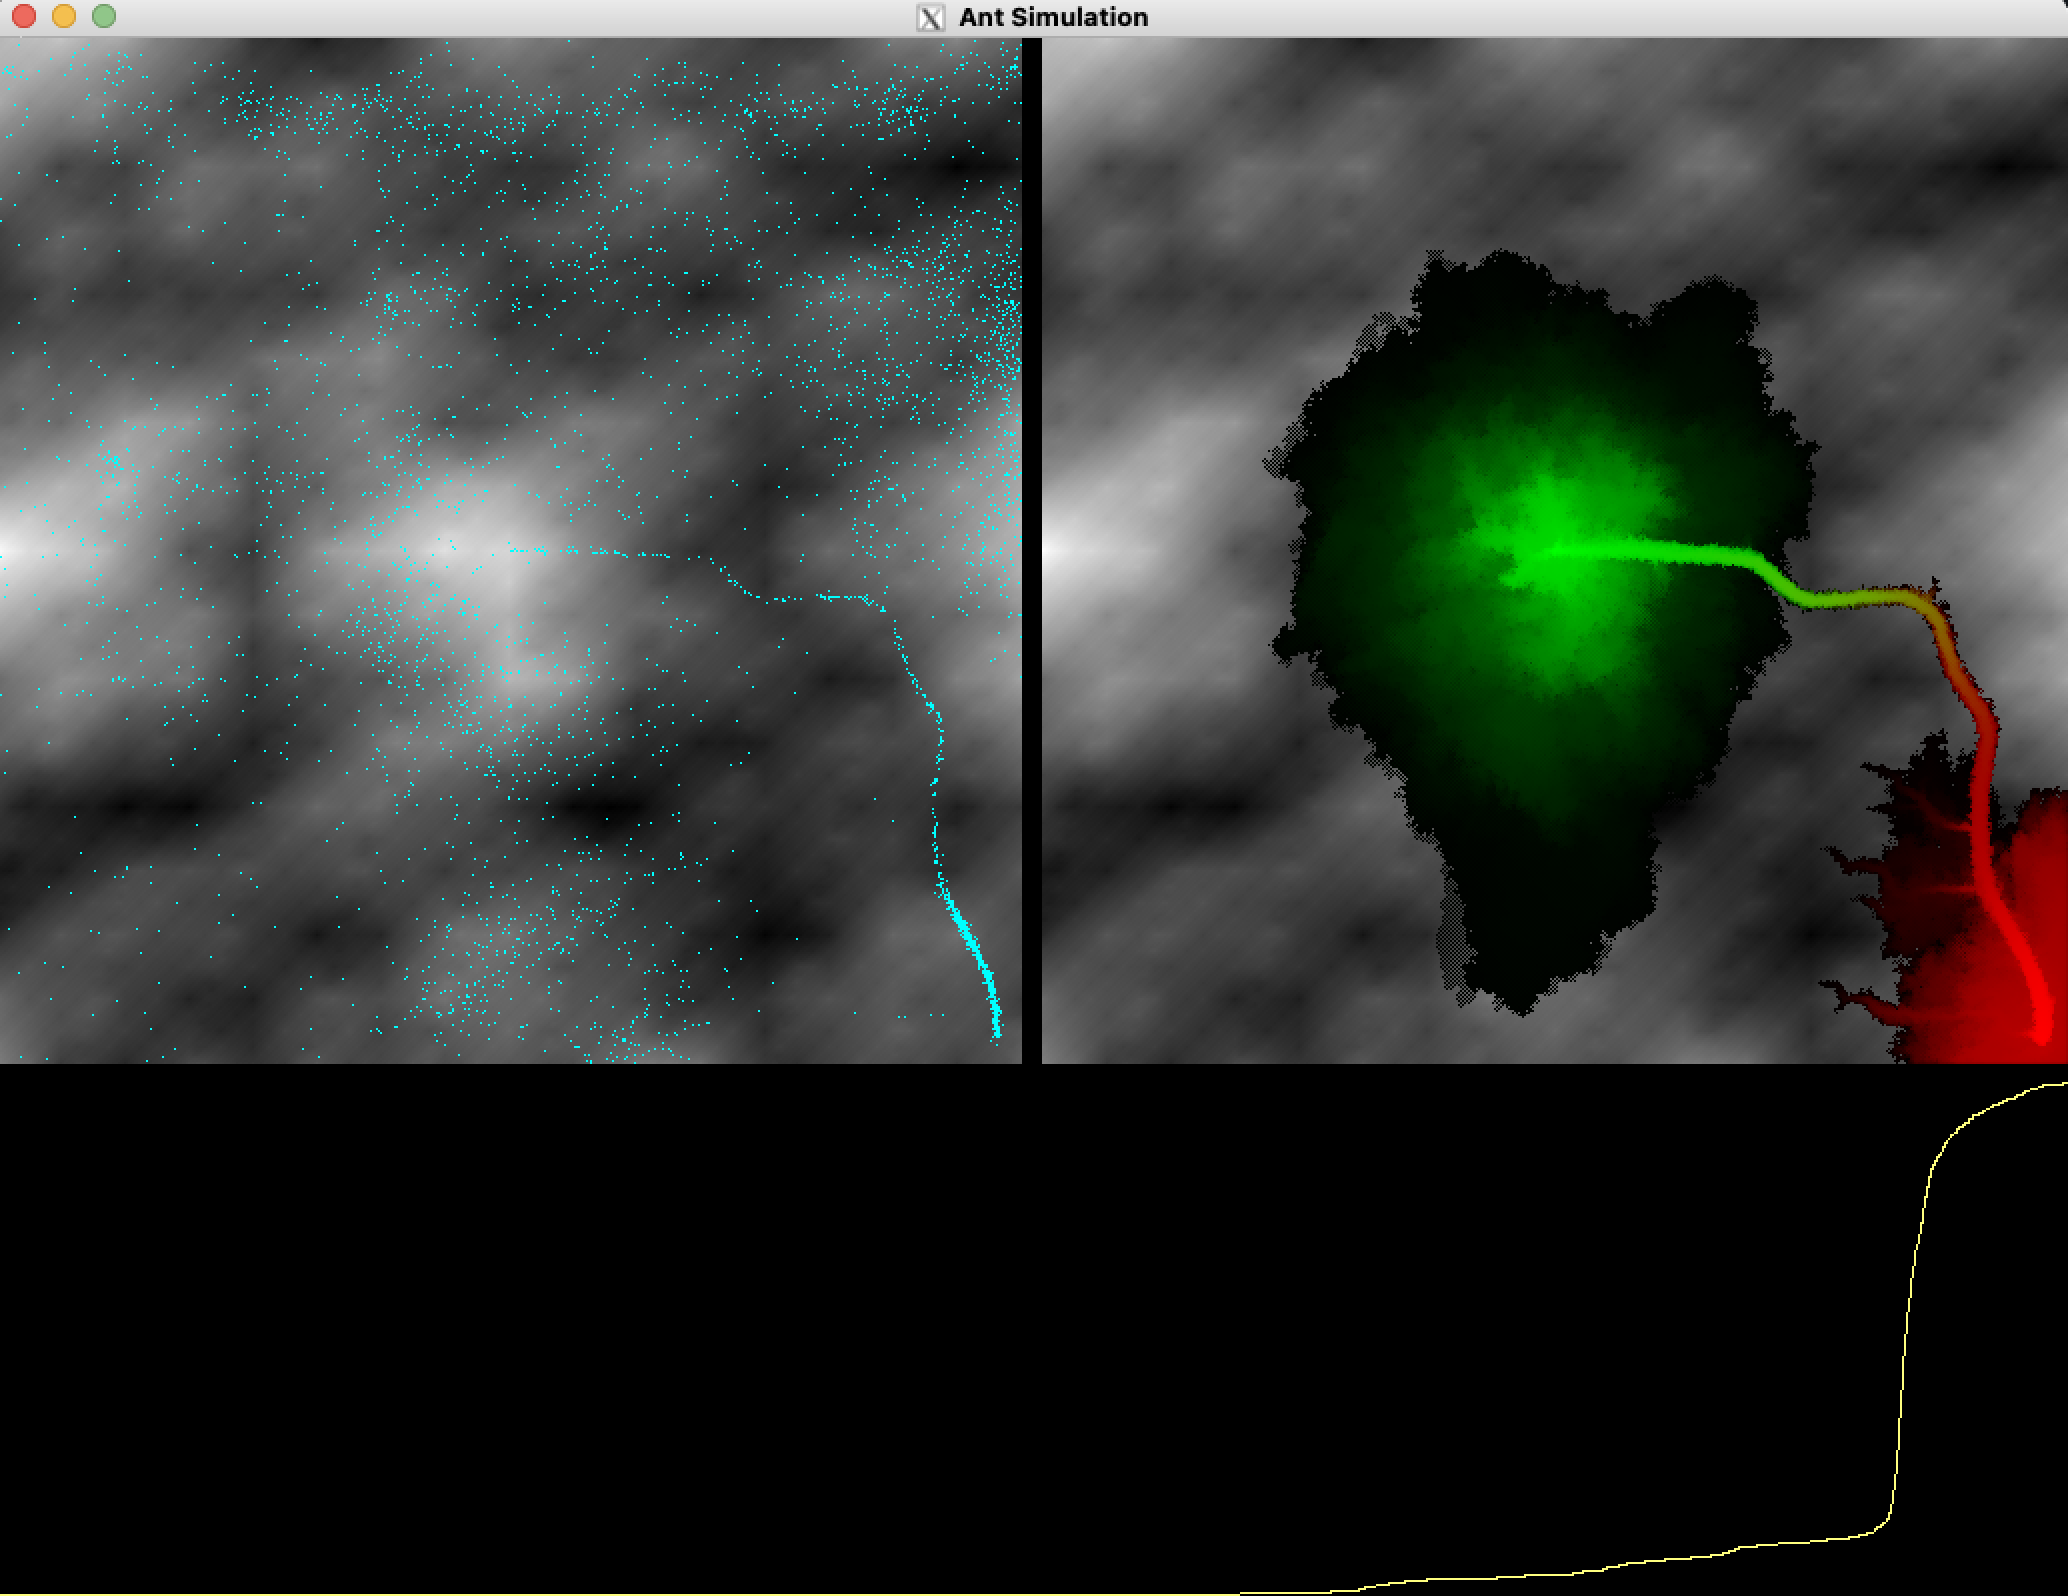
\includegraphics[width=0.82\textwidth]{Ant_Simulation.png}
    \caption{Interface graphique de la simulation ACO après convergence (513$\times$513, 5000 fourmis).
    \textbf{Gauche} : terrain fractal en niveaux de gris, points cyan = fourmis en exploration.
    \textbf{Droite} : carte de phéromones superposée — vert = phéromones de retour au nid
    (depuis la nourriture), rouge = phéromones d'aller (depuis le nid) ; la concentration
    élevée révèle le chemin optimal convergé.
    \textbf{Bas} : courbe jaune de collecte cumulée, montrant la phase d'exploration plate puis la montée abrupte après découverte du chemin (itération 2942).}
    \label{fig:gui}
\end{figure}


\subsection{Protocole de mesure}

Le code est instrumenté avec \texttt{std::chrono::high\_resolution\_clock} pour mesurer séparément : l'avancement des fourmis, l'évaporation ($\times\beta$) et la mise à jour des buffers. Le mode \texttt{-{}-headless} désactive le rendu SDL (qui représente 86\% du temps en mode graphique) pour mesurer uniquement le calcul.




\subsection{Baseline séquentielle}

\begin{table}[H]
\centering
\begin{tabular}{lrrr}
\toprule
\textbf{Composant} & \textbf{Temps (ms)} & \textbf{ms/iter} & \textbf{Proportion} \\
\midrule
Avancement fourmis     & 8491.60  & 1.70 & 93.81\% \\
Évaporation phéromones & 556.60   & 0.11 & 6.15\% \\
Mise à jour buffers    & 4.40     & 0.00 & 0.05\% \\
\midrule
\textbf{Total boucle}  & \textbf{9051.20} & \textbf{1.81} & \textbf{100\%} \\
\bottomrule
\end{tabular}
\caption{Baseline séquentielle --- médiane de 3 exécutions, 5000 itérations}
\label{tab:baseline}
\end{table}

La stabilité des mesures est excellente : sur les 3 exécutions, l'écart-type du temps total est de 9.30 ms (CV = 0.10\%). Les résultats fonctionnels sont strictement identiques : première nourriture à l'itération 2942, total de 2440 unités collectées, confirmant le déterminisme du générateur pseudo-aléatoire (graine fixe 2026).

\begin{formal}
L'avancement des fourmis domine à 93.81\% du temps. Chaque fourmi effectue plusieurs déplacements par pas de temps (boucle \texttt{while(consumed\_time < 1.)}) avec des accès mémoire dispersés dans la carte de phéromones (4.20 Mo), qui dépasse le cache L2 ($\sim$256 Ko par c\oe ur). Ce composant est la cible prioritaire de toute optimisation.
\end{formal}

\newpage
% ============================================================
\section{Vectorisation --- Restructuration AoS $\to$ SoA}

\subsection{Principe}

Dans la version originale (AoS), chaque fourmi est un objet \texttt{ant} contenant \texttt{\{seed, state, position\}}. Les 5000 objets sont stockés dans un \texttt{std::vector<ant>}. La restructuration SoA sépare les attributs en tableaux parallèles :

\begin{lstlisting}[language=C++, caption={Structure SoA}]
struct ants_soa {
    std::vector<int> positions_x, positions_y;
    std::vector<unsigned char> states;
    std::vector<std::size_t> seeds;
    std::size_t count;
};
\end{lstlisting}

Chaque tableau est parcouru séquentiellement, ce qui maximise l'utilisation des lignes de cache (16 \texttt{int}/ligne pour les positions, 8 \texttt{size\_t}/ligne pour les graines).

\subsection{Résultats}

\begin{table}[H]
\centering
\begin{tabular}{lrrrr}
\toprule
\textbf{Composant} & \textbf{AoS (ms)} & \textbf{SoA (ms)} & \textbf{Diff.} & \textbf{Accél.} \\
\midrule
Avancement fourmis       & 8495.50 & 8441.50 & $-54.00$ & 1.01$\times$ \\
Évaporation              & 567.10  & 555.80  & $-11.30$ & 1.02$\times$ \\
\textbf{Total boucle}    & \textbf{9067.00} & \textbf{9003.00} & \textbf{$-64.00$} & \textbf{1.01$\times$} \\
\bottomrule
\end{tabular}
\caption{Comparaison AoS vs SoA (médiane, 5000 itérations)}
\label{tab:soa}
\end{table}

Les deux versions SoA et AoS montrent un coefficient de variation inférieur à 0.10\%, confirmant la stabilité des mesures. La reproductibilité fonctionnelle est parfaite entre les deux versions (itération 2942, 2440 unités).

\subsection{Analyse du gain marginal}

Le gain de 0.71\% est statistiquement réel (supérieur au bruit de mesure, CV < 0.10\%) mais pratiquement négligeable. L'explication tient au profil d'accès mémoire :

\begin{itemize}[nosep]
    \item Le goulot d'étranglement est l'accès aux \textbf{phéromones} (4.20 Mo, accès aléatoires), pas la disposition des fourmis ($\sim$120 Ko en AoS, $\sim$100 Ko en SoA : les deux tiennent dans le cache L2). L'objet \texttt{ant} original est compact ($\sim$24 octets) : une ligne de cache (64 octets) contient 2--3 fourmis, le gaspillage est limité.
    \item L'algorithme suit un schéma \emph{scatter/gather} (chaque fourmi lit une position aléatoire dans les phéromones) et non un schéma \emph{stream}, où la SoA excelle. La boucle interne a un nombre variable d'itérations par fourmi (dépendant de la valeur du terrain), empêchant la vectorisation SIMD par le compilateur.
\end{itemize}

\begin{formal}
Ce résultat négatif est en soi informatif : il démontre que toute restructuration mémoire n'améliore pas automatiquement les performances. Le vrai levier est la \textbf{parallélisation}. Néanmoins, la restructuration SoA facilite le partitionnement des fourmis entre threads OpenMP et réduit le risque de \emph{false sharing}.
\end{formal}

\newpage
% ============================================================
\section{Parallélisation OpenMP (mémoire partagée)}

\subsection{Stratégie}

Deux régions parallèles sont introduites :

\subsubsection{Avancement des fourmis (93.8\%)}

\begin{lstlisting}[language=C++, caption={Parallélisation de l'avancement des fourmis}]
#pragma omp parallel for schedule(dynamic, 50) reduction(+:local_food)
for (size_t i = 0; i < ants.count; ++i) {
    // advance ant i ...
}
\end{lstlisting}

L'ordonnancement dynamique est choisi car le nombre de pas par fourmi varie selon le terrain. Les écritures concurrentes dans le buffer de phéromones (\texttt{mark\_pheronome}) sont tolérées sans protection atomique (méthode C) : la probabilité de collision est faible ($\sim$4.70\% par itération pour 5000 fourmis sur $513^2$ cellules), et l'algorithme est intrinsèquement stochastique.

\subsubsection{Évaporation des phéromones (6.2\%)}

\begin{lstlisting}[language=C++, caption={Évaporation parallèle}]
#pragma omp parallel for collapse(2) schedule(static)
for (size_t i = 1; i <= dim; ++i)
    for (size_t j = 1; j <= dim; ++j)
        // evaporate cell (i,j)
\end{lstlisting}

Boucle parfaitement parallèle ($513^2 \approx 263\,000$ itérations indépendantes).

\subsection{Résultats}

\begin{table}[H]
\centering
\begin{tabular}{rrrrrrrr}
\toprule
\textbf{Threads} & \textbf{Fourmis} & \textbf{Évap.} & \textbf{M. à j.} & \textbf{Total (ms)} & $\boldsymbol{S(p)}$ & $\boldsymbol{E(p)}$ & \textbf{Nourr.} \\
\midrule
1  & 8367.60  & 735.00  & 4.40   & 9107.10  & 1.00$\times$ & 100\%  & 2440 \\
2  & 4290.10  & 414.80  & 7.40   & 4720.50  & 1.93$\times$ & 96.50\% & 2440 \\
4  & 2236.70  & 266.60  & 9.60   & 2508.00  & 3.63$\times$ & 90.80\% & 2440 \\
8  & 1364.20  & 299.00  & 14.80  & 1678.20  & 5.43$\times$ & 67.80\% & 2440 \\
12 & 2190.10  & 1187.40 & 22.50  & 3400.80  & 2.68$\times$ & 22.30\% & 2440 \\
\bottomrule
\end{tabular}
\caption{Passage à l'échelle OpenMP (médiane, 5000 itérations)}
\label{tab:omp}
\end{table}

\begin{figure}[H]
    \centering
    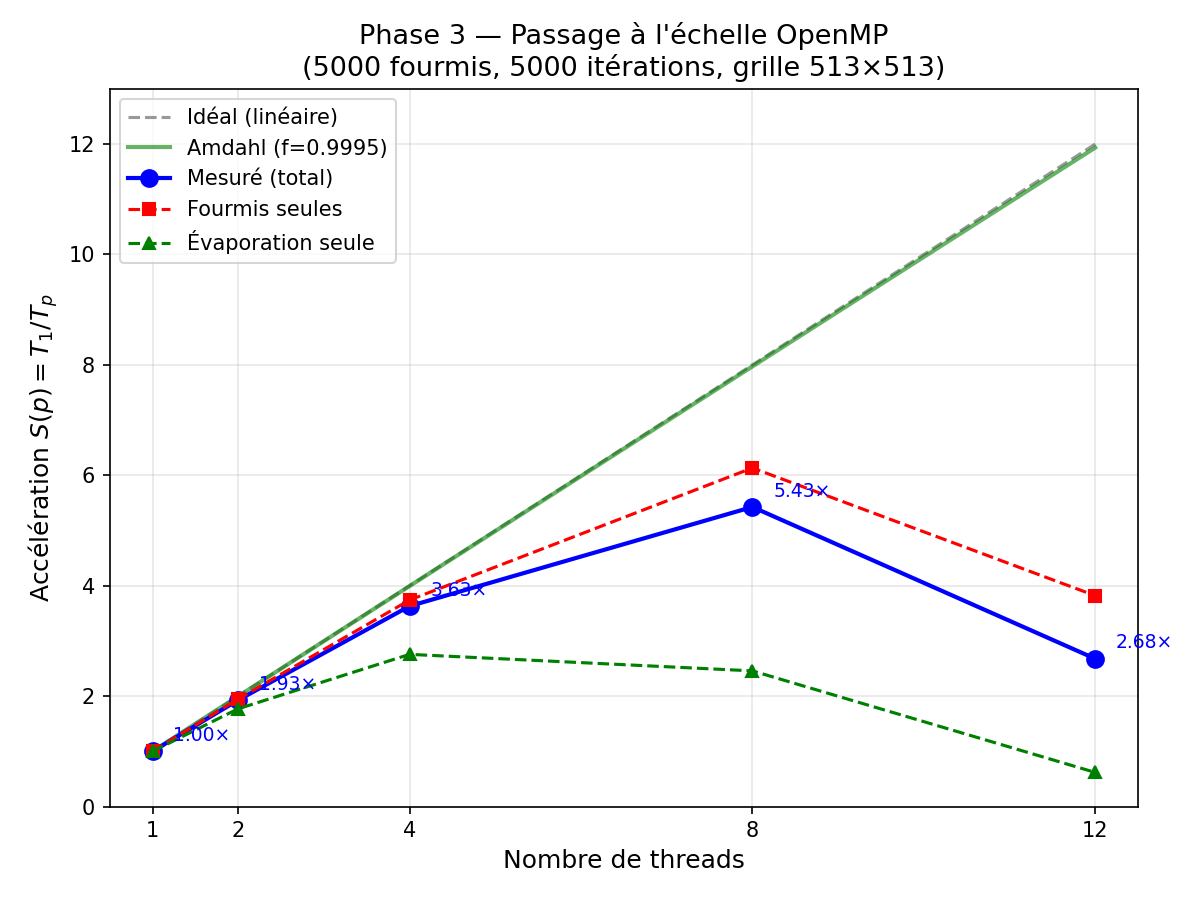
\includegraphics[width=0.75\textwidth]{omp_speedup.png}
    \caption{Accélération OpenMP : mesurée vs loi d'Amdahl vs linéaire idéale}
    \label{fig:omp_speedup}
\end{figure}

\begin{figure}[H]
    \centering
    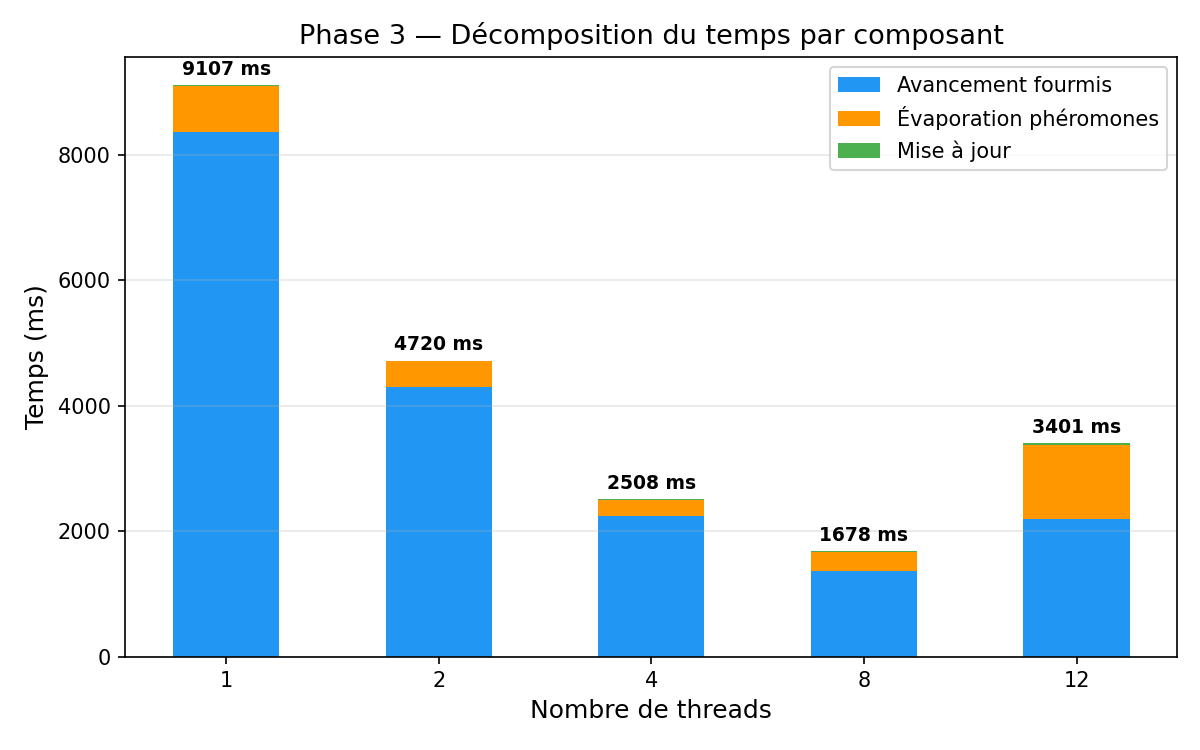
\includegraphics[width=0.75\textwidth]{omp_breakdown.png}
    \caption{Décomposition du temps par composant en fonction du nombre de threads}
    \label{fig:omp_breakdown}
\end{figure}

\subsection{Analyse}

\subsubsection{Accélération maximale à 8 threads : $5.43\times$}

Le meilleur résultat est obtenu avec 8 threads, réduisant le temps de 9107 ms à 1678 ms. L'avancement des fourmis atteint $S_\text{fourmis}(8) = 6.13\times$, confirmant l'efficacité du \texttt{schedule(dynamic)}.

La variabilité des mesures augmente avec le nombre de threads : le CV passe de 0.09\% (1T) à 10.90\% (8T), ce qui reflète la contention croissante pour les ressources partagées.

\subsubsection{Régression à 12 threads}

La performance chute à $2.68\times$ pour 12 threads. Trois facteurs convergent :

\begin{enumerate}[nosep]
    \item \textbf{Saturation de la bande passante mémoire} : l'évaporation, kernel \emph{memory-bound} (1 multiplication par lecture/écriture de 8 octets), passe de 299.00 ms (8T) à 1187.40 ms (12T) --- soit $1.62\times$ \emph{plus lent qu'en séquentiel}.
    \item \textbf{Contention du cache L2/L3} : la carte de phéromones (4.20 Mo) provoque du \emph{thrashing} avec 12 threads accédant simultanément.
    \item \textbf{Overhead d'ordonnancement} : $\lceil 5000/50 \rceil = 100$ tâches dynamiques par itération, avec barrières de synchronisation croissantes.
\end{enumerate}

\subsubsection{Transfert de goulot d'étranglement}

La proportion de l'évaporation passe de 8.10\% (1T) à 34.90\% (12T). Résoudre le goulot des fourmis en révèle un autre sur l'évaporation.

\subsubsection{Comparaison avec la loi d'Amdahl}

Avec une fraction parallélisable $f = (8367.60 + 735.00) / 9107.10 = 0.9995$, la loi d'Amdahl prédit $S(8) = 7.96\times$ et $S(12) = 11.9\times$, alors que les mesures donnent respectivement $5.43\times$ et $2.68\times$. L'écart croissant démontre que le modèle d'Amdahl, qui ignore la contention mémoire et l'overhead de parallélisation, est trop optimiste pour ce type de charge \emph{memory-bound}.

\subsubsection{Reproductibilité}

Les 15 exécutions (5 configs $\times$ 3 runs) produisent des résultats fonctionnels identiques (itération 2942, 2440 unités), confirmant que la tolérance aux conditions de course n'affecte pas la convergence. La probabilité de collision par itération reste faible : $P \approx m^2 / (2N) \approx 4.7\%$ pour 5000 fourmis sur $513^2$ cellules.

\begin{figure}[H]
    \centering
    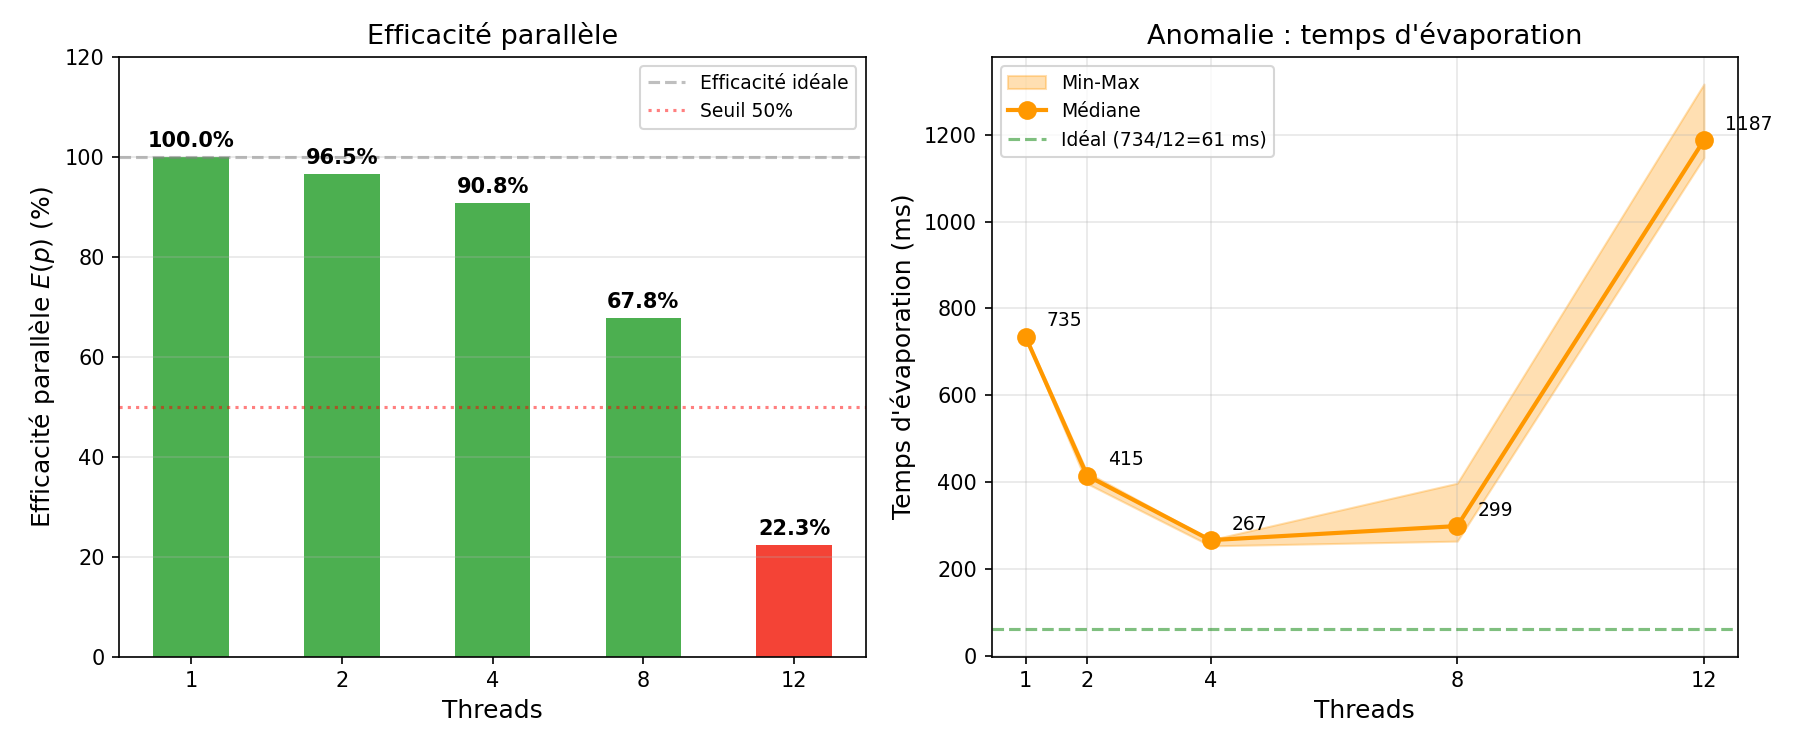
\includegraphics[width=0.9\textwidth]{omp_efficiency.png}
    \caption{Efficacité parallèle et anomalie du temps d'évaporation}
    \label{fig:omp_efficiency}
\end{figure}

\newpage
% ============================================================
\section{Parallélisation MPI --- Méthode 1 (réplication de la carte)}

\subsection{Conception}

Chaque processus conserve une copie complète de la carte ($513 \times 513$) et gère $\lfloor m/P \rfloor$ fourmis. La synchronisation suit le schéma :

\begin{enumerate}[nosep]
    \item Avancement des fourmis locales ($N/P$ fourmis)
    \item \texttt{MPI\_Allreduce(MPI\_MAX)} sur le buffer de phéromones ($\sim$4.24 Mo)
    \item Évaporation distribuée par blocs de lignes + \texttt{MPI\_Allgatherv} ($\sim$4.23 Mo)
    \item \texttt{phen.update()} (échange de buffers)
\end{enumerate}

La sémantique \texttt{MPI\_MAX} est correcte car \texttt{mark\_pheronome} ne fait qu'augmenter les valeurs (marquage = 1.0), conformément au cahier des charges.

\subsection{Volume de communication}

Le volume total par itération est de $\sim$\textbf{8.50 Mo} (4.24 Mo pour \texttt{Allreduce} + 4.23 Mo pour \texttt{Allgatherv}), \textbf{indépendant} du nombre de processus.

\subsection{Résultats}

\begin{table}[H]
\centering
\begin{tabular}{rrrrrrrr}
\toprule
$\boldsymbol{P}$ & \textbf{Fourmis} & \textbf{Comm.} & \textbf{Évap.} & \textbf{Total (ms)} & $\boldsymbol{S(P)}$ & $\boldsymbol{E(P)}$ & \textbf{Nourr.} \\
\midrule
1  & 8540.10  & 764.70    & 1114.00  & 10423.50  & 1.00$\times$ & 100\%  & 2440 \\
2  & 4607.40  & 3060.90   & 1602.10  & 9323.80   & 1.12$\times$ & 55.90\% & 2651 \\
4  & 2634.00  & 5266.10   & 3639.80  & 11655.30  & 0.89$\times$ & 22.40\% & 2651 \\
8  & 1717.80  & 16093.00  & 8628.60  & 27887.40  & 0.37$\times$ & 4.70\%  & 2651 \\
12 & 1713.60  & 67392.70  & 32466.80 & 112636.50 & 0.09$\times$ & 0.80\% & 2651 \\
\bottomrule
\end{tabular}
\caption{Passage à l'échelle MPI méthode 1 (médiane, 5000 itérations)}
\label{tab:mpi1}
\end{table}

\begin{figure}[H]
    \centering
    \begin{subfigure}[t]{0.48\textwidth}
        \centering
        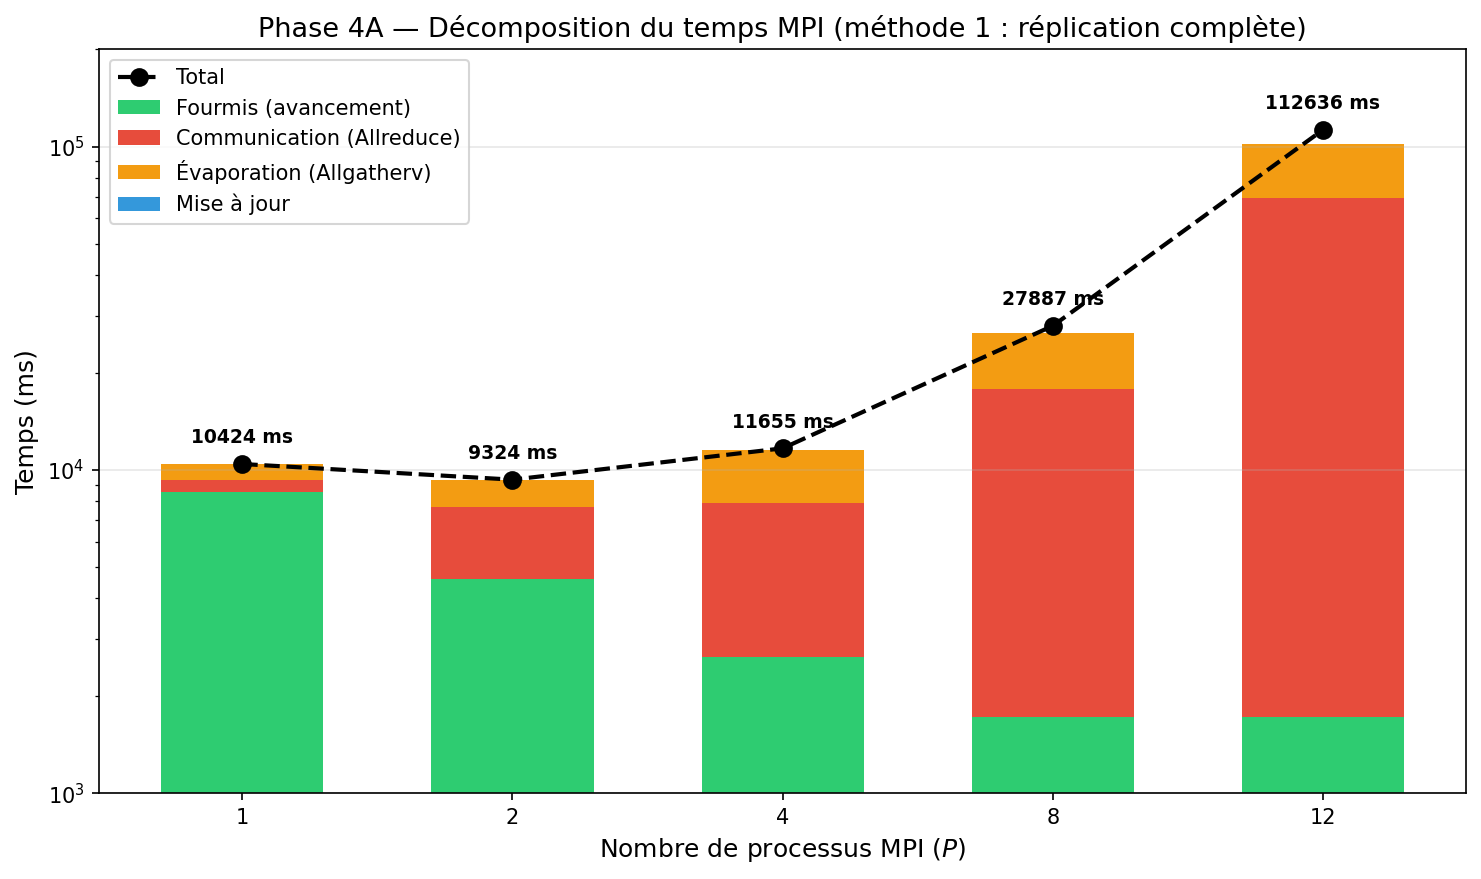
\includegraphics[width=\textwidth]{mpi_scaling_chart.png}
        \caption{Temps total et décomposition}
        \label{fig:mpi1_scaling}
    \end{subfigure}
    \hfill
    \begin{subfigure}[t]{0.48\textwidth}
        \centering
        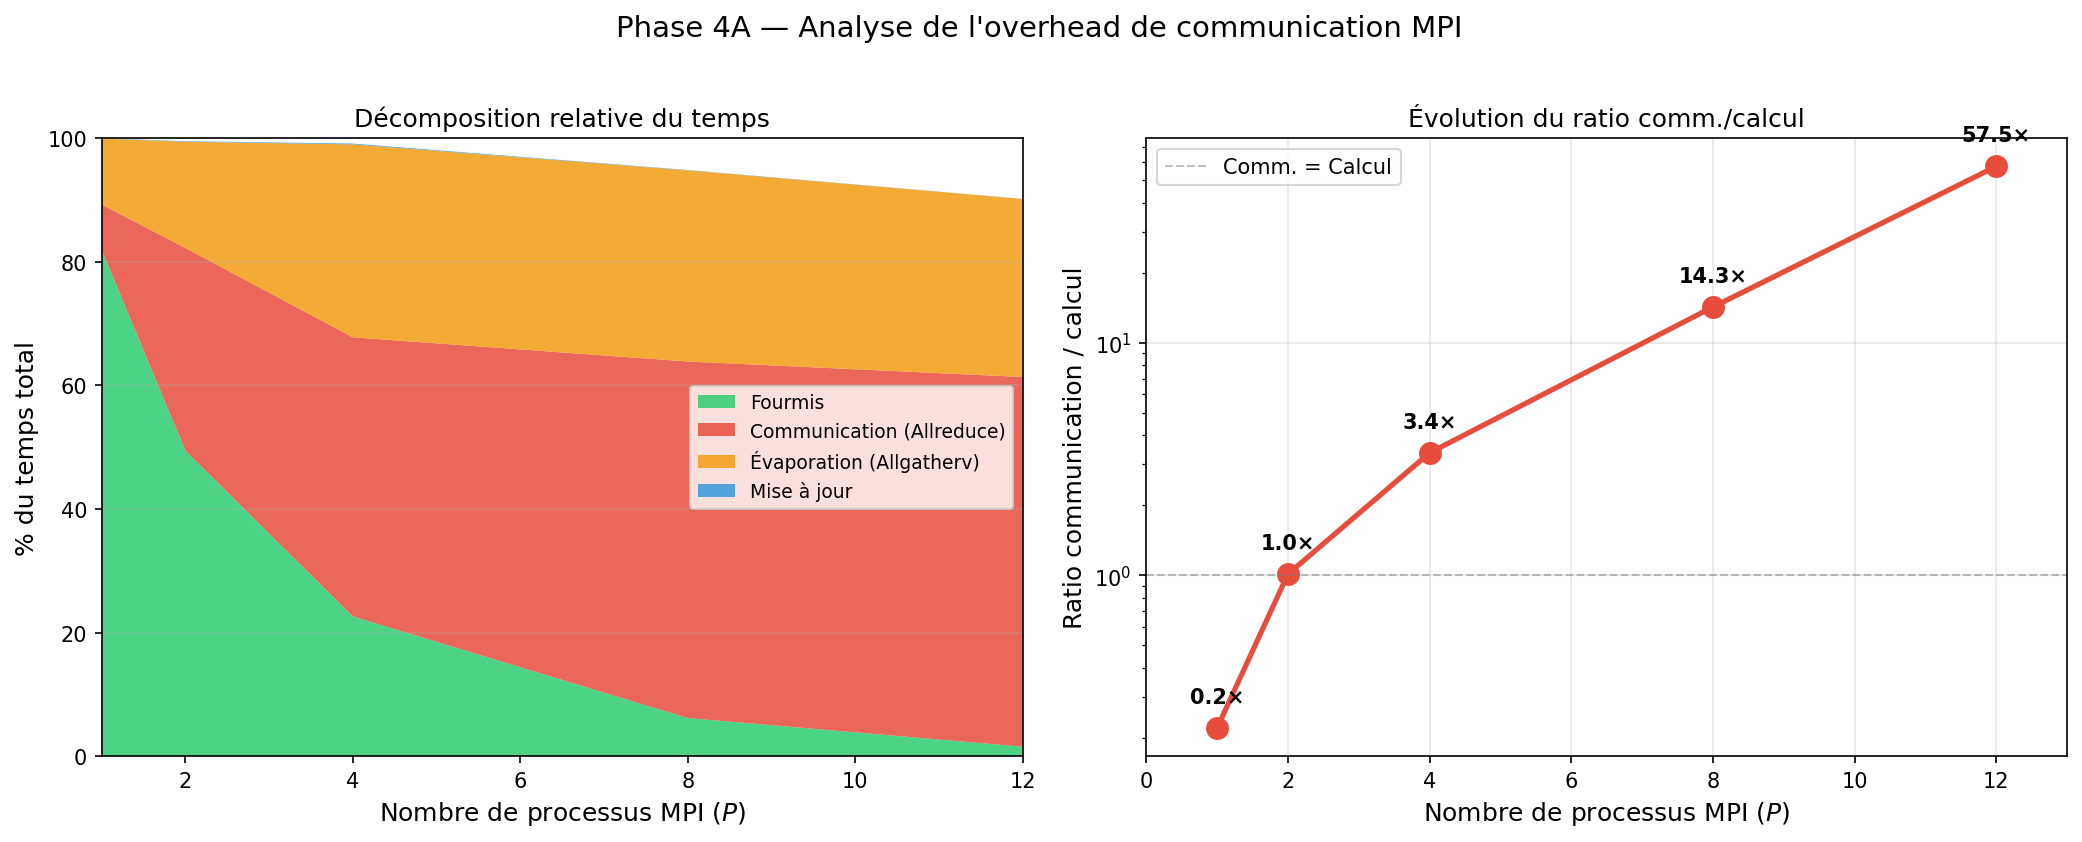
\includegraphics[width=\textwidth]{mpi_comm_ratio.png}
        \caption{Ratio communication / calcul}
        \label{fig:mpi1_comm}
    \end{subfigure}
    \caption{MPI méthode 1 --- passage à l'échelle et ratio de communication}
\end{figure}

\subsection{Analyse}

La méthode 1 est \textbf{contre-productive} au-delà de 2 processus. L'accélération maximale n'est que de $1.12\times$ ($P=2$) et le programme est $11\times$ plus lent à $P=12$.

Le ratio communication/calcul explose : il passe de 0.08 ($P=1$) à 57.55 ($P=12$). Le volume de 8.50 Mo par itération est \textbf{constant} quel que soit $P$, car chaque processus synchronise la totalité de la carte. Ajouter des processus réduit le calcul mais augmente le coût des opérations collectives ($O(\log P)$ étapes avec volume total inchangé, plus contention sur le bus mémoire).

L'avancement des fourmis seul passe à l'échelle correctement ($S_\text{fourmis}(8) = 4.97\times$), ce qui confirme que le partitionnement du travail est efficace --- mais ce gain est totalement absorbé par la communication.

Le mode hybride MPI+OpenMP a aussi été testé (cf. tableau~\ref{tab:mpi1_hybrid}) : la configuration $P=1, T=8$ produit 10434.50 ms, soit 14\% plus lent que le pur OpenMP 8 threads (1678.20 ms). L'overhead provient de la couche MPI (\texttt{MPI\_Allreduce} + \texttt{MPI\_Allgatherv}) qui subsiste même avec un seul processus.

\begin{table}[H]
\centering
\begin{tabular}{rrrrrr}
\toprule
$\boldsymbol{P}$ & $\boldsymbol{T}$ & \textbf{Cœurs} & \textbf{Total (ms)} & $\boldsymbol{S_\text{seq}}$ & \textbf{Nourr.} \\
\midrule
1 & 8  & 8  & 10434.50  & 0.87$\times$ & 2440 \\
2 & 4  & 8  & 9339.70   & 0.98$\times$ & 2651 \\
4 & 2  & 8  & 10884.60  & 0.84$\times$ & 2651 \\
2 & 2  & 4  & 8964.50   & 1.02$\times$ & 2651 \\
4 & 1  & 4  & 11090.40  & 0.82$\times$ & 2651 \\
\bottomrule
\end{tabular}
\caption{Mode hybride MPI méthode 1 + OpenMP ($S_\text{seq} = 9107.10 / T_\text{hybrid}$)}
\label{tab:mpi1_hybrid}
\end{table}

\begin{formal}
\textbf{Conclusion :} la parallélisation MPI avec réplication de la carte échoue pour cette configuration. Le ratio calcul/communication est trop défavorable : la grille $513 \times 513$ génère 8.50 Mo de données collectives par itération, indépendamment du nombre de processus. Ce résultat négatif est conforme à la prédiction du cahier des charges et illustre que la parallélisation distribuée n'est pas toujours bénéfique.
\end{formal}

\newpage
% ============================================================
\section{Parallélisation MPI --- Méthode 2 (partitionnement de la carte)}

\subsection{Conception}

\subsubsection{Décomposition 1D par lignes}

La grille est découpée en bandes horizontales. Chaque processus $r$ possède $\lfloor 513/P \rfloor$ ou $\lceil 513/P \rceil$ lignes, avec une rangée de cellules fantômes (ghost cells) en haut et en bas.

\begin{figure}[H]
\centering
\begin{verbatim}
             
    0                                   512    Y
  0  +-----------------------------------+
     |       Rank 0  (~128 lignes)       |
     |  ghost                            |
 128 +-----------------------------------+
     |       Rank 1  (~129 lignes)       |
     |  ghost                            |
 257 +-----------------------------------+
     |       Rank 2  (~128 lignes)       |
     |  ghost                            |
 385 +-----------------------------------+
     | Rank 3  (~128 lignes)             |
     |                                   |
 512 +-----------------------------------+

  X
\end{verbatim}
\caption*{Décomposition 1D pour $P=4$ processus}
\end{figure}

\subsubsection{Schéma de communication par itération}

\begin{enumerate}[nosep]
    \item Avancement des fourmis locales, détection des dépassements de frontière
    \item \textbf{Migration des fourmis} : protocole en 2 étapes via \texttt{MPI\_Sendrecv} (échange des compteurs, puis des données)
    \item \textbf{Halo exchange} : échange bidirectionnel des lignes de bordure ($\sim$8 Ko par direction)
    \item \textbf{Fusion MAX} des phéromones aux frontières
    \item Évaporation locale + mise à jour des buffers
\end{enumerate}

\subsubsection{Réduction du volume de communication}

\begin{table}[H]
\centering
\begin{tabular}{lrrr}
\toprule
\textbf{Communication} & \textbf{Méthode 1} & \textbf{Méthode 2} & \textbf{Réduction} \\
\midrule
Phéromones (sync)    & 4.24 Mo (\texttt{Allreduce})   & $\sim$32 Ko (halo)    & $\times 132$ \\
Évaporation          & 4.23 Mo (\texttt{Allgatherv})   & 0 (locale)            & $\infty$    \\
Migration fourmis    & 0                               & quelques Ko            & nouveau     \\
\midrule
\textbf{Total/iter}  & \textbf{$\sim$8.50 Mo}          & \textbf{$\sim$50 Ko}  & $\boldsymbol{\times 170}$ \\
\bottomrule
\end{tabular}
\caption{Volume de communication : méthode 1 vs méthode 2}
\label{tab:comm_volume}
\end{table}

\subsection{Résultats --- MPI méthode 2 pur}

\begin{table}[H]
\centering
\begin{tabular}{rrrrrrrrr}
\toprule
$\boldsymbol{P}$ & \textbf{Fourmis} & \textbf{Comm.} & \textbf{Évap.} & \textbf{M. à j.} & \textbf{Total (ms)} & $\boldsymbol{S(P)}$ & $\boldsymbol{E(P)}$ & \textbf{Nourr.} \\
\midrule
1  & 8354.70  & 2.00      & 475.00   & 5.50    & 8881.40  & 1.00$\times$ & 100\%  & 2440 \\
2  & 3069.40  & 2345.40   & 222.40   & 74.30   & 5721.90  & 1.55$\times$ & 77.60\% & 2092 \\
4  & 1146.30  & 2123.80   & 101.20   & 61.90   & 3443.80  & 2.58$\times$ & 64.50\% & 3609 \\
8  & 371.20   & 1991.70   & 65.60    & 458.40  & 3216.50  & 2.76$\times$ & 34.50\% & 3445 \\
12 & 280.30   & 16774.90  & 77.20    & 6999.80 & 39814.60 & 0.22$\times$ & 1.90\%  & 3670 \\
\bottomrule
\end{tabular}
\caption{Passage à l'échelle MPI méthode 2 (médiane, 5000 itérations)}
\label{tab:mpi2}
\end{table}

\begin{figure}[H]
    \centering
    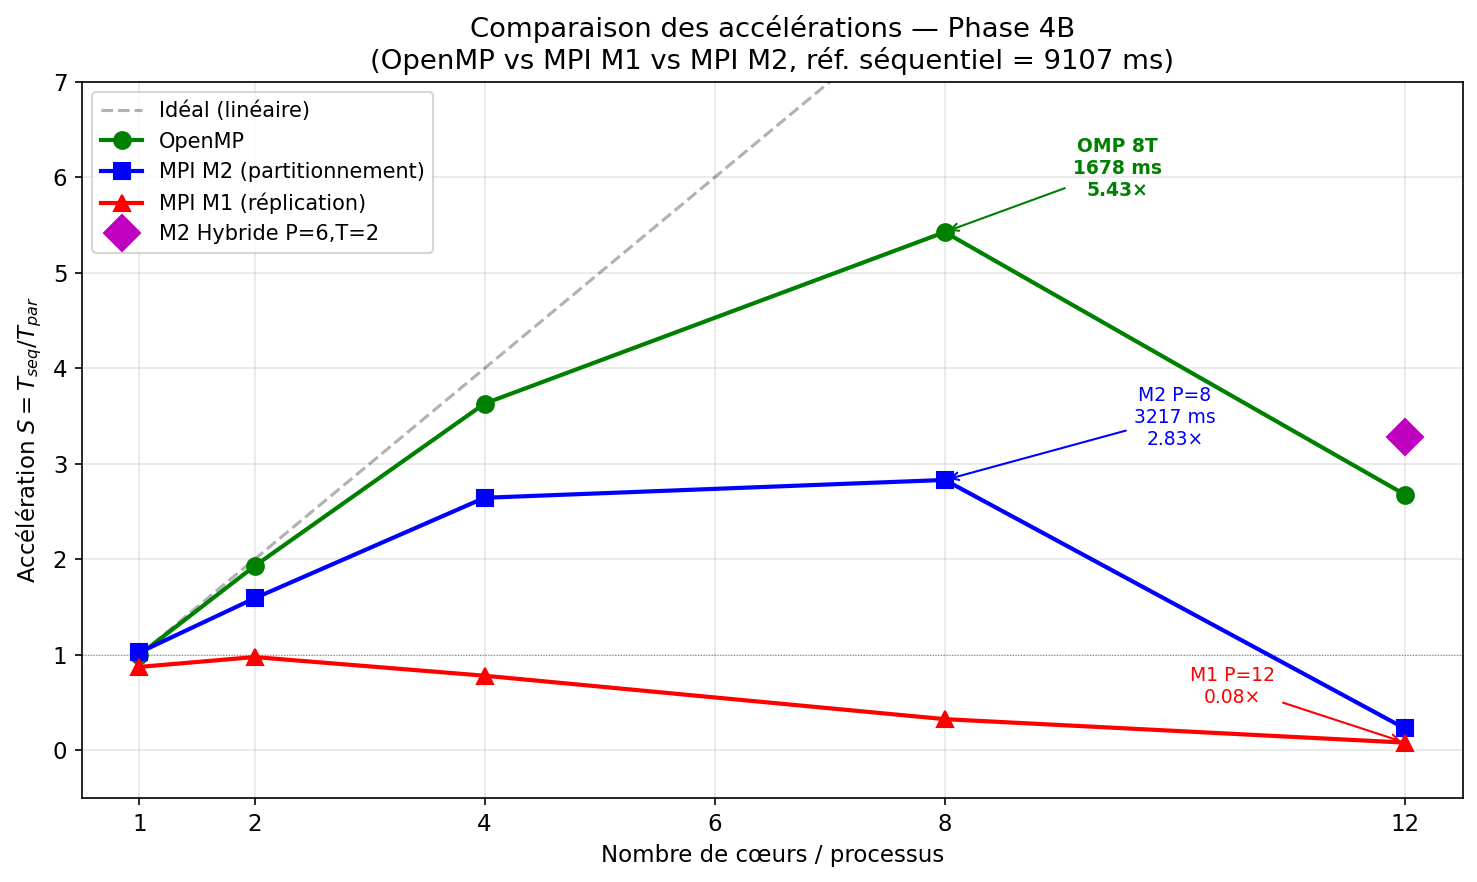
\includegraphics[width=0.78\textwidth]{mpi2_speedup_comparison.png}
    \caption{Accélération comparée : OpenMP vs MPI M1 vs MPI M2}
    \label{fig:mpi2_speedup}
\end{figure}

\begin{figure}[H]
    \centering
    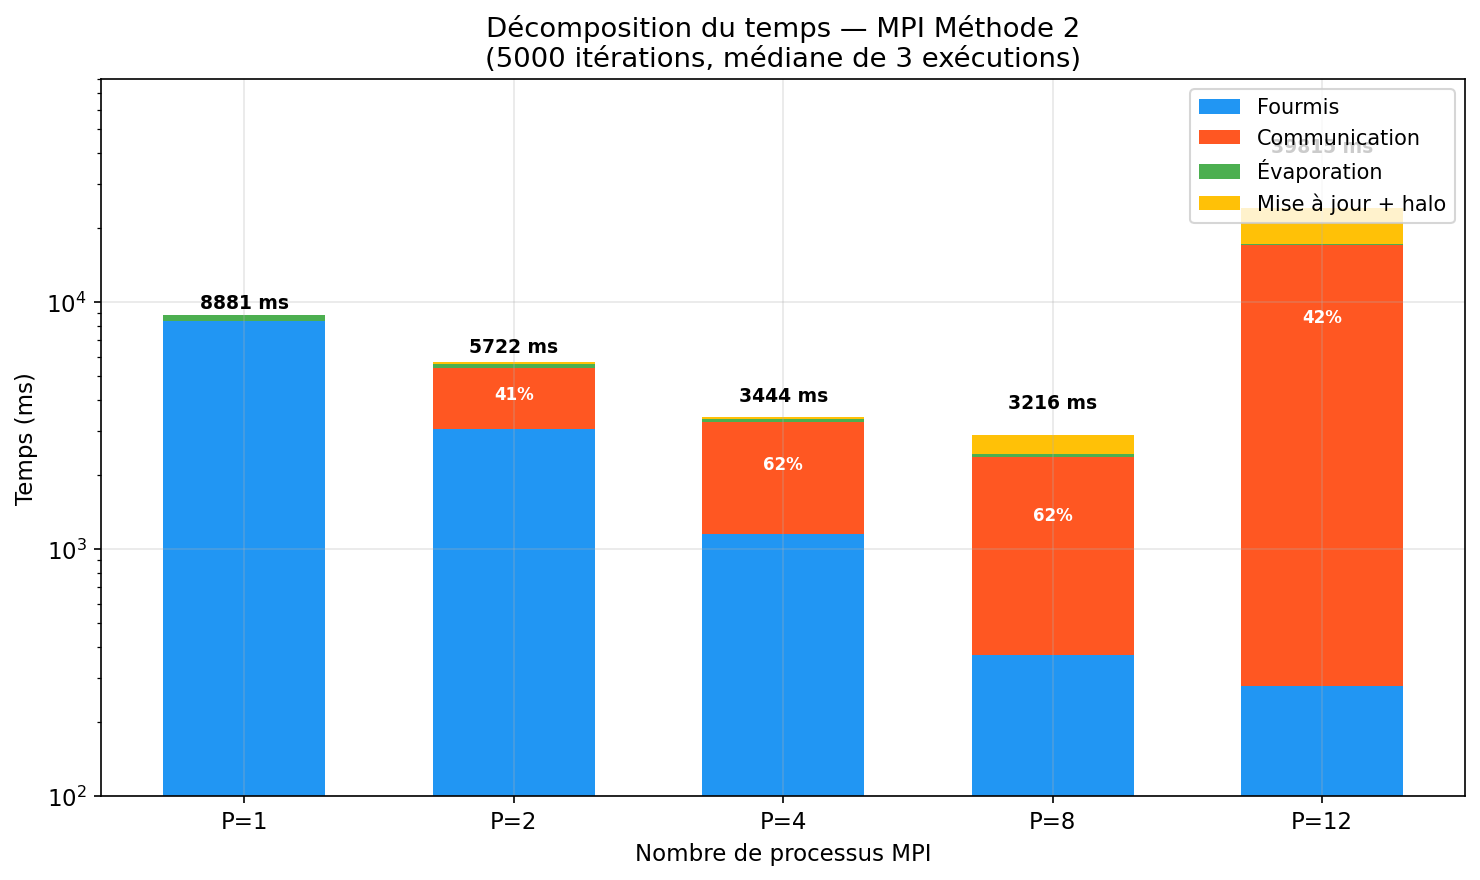
\includegraphics[width=0.78\textwidth]{mpi2_time_breakdown.png}
    \caption{Décomposition du temps --- MPI méthode 2}
    \label{fig:mpi2_breakdown}
\end{figure}

\subsection{Accélération super-linéaire des fourmis}

Le résultat le plus remarquable concerne l'accélération du seul composant ``fourmis'' :

\begin{table}[H]
\centering
\begin{tabular}{rrrr}
\toprule
$\boldsymbol{P}$ & \textbf{Fourmis (ms)} & $\boldsymbol{S_\text{fourmis}(P)}$ & \textbf{Carte locale} \\
\midrule
1  & 8354.70  & 1.00$\times$   & 4.20 Mo \\
2  & 3069.40  & 2.72$\times$   & 2.10 Mo \\
4  & 1146.30  & 7.29$\times$   & 1.07 Mo \\
8  & 371.20   & 22.51$\times$  & 0.55 Mo \\
12 & 280.30   & 29.81$\times$  & 0.37 Mo \\
\bottomrule
\end{tabular}
\caption{Accélération super-linéaire du composant ``fourmis'' --- effet de cache}
\label{tab:superlinear}
\end{table}

Pour $P = 8$, la carte locale (0.55 Mo) tient dans le cache L2 ($\sim$256 Ko pour les accès fréquents), éliminant les \emph{cache misses} qui dominent l'accès au tableau complet de 4.20 Mo. Combiné à la réduction du nombre de fourmis par processus, cela produit une efficacité de 281\% --- un avantage structurel de la méthode 2 que la méthode 1 ne peut pas atteindre.

\subsection{Déséquilibre de charge}

\begin{table}[H]
\centering
\begin{tabular}{llr}
\toprule
$\boldsymbol{P}$ & \textbf{Distribution des fourmis} & \textbf{Ratio max/min} \\
\midrule
2  & R0=1340, \textbf{R1=3660}           & $2.73\times$ \\
4  & R0=303, R1=1342, R2=1376, \textbf{R3=1979} & $6.53\times$ \\
8  & R0=125, \ldots, \textbf{R7=1435}    & $11.48\times$ \\
12 & R0=33, \ldots, \textbf{R11=1349}    & $40.88\times$ \\
\bottomrule
\end{tabular}
\caption{Distribution finale des fourmis et ratio de déséquilibre}
\label{tab:load_imbalance}
\end{table}

La source de nourriture $(500,500)$ est toujours dans le dernier processus, qui accumule le plus de fourmis après convergence. Le ratio max/min atteint $40.88\times$ pour $P=12$, rendant le parallélisme inefficace : les processus rapides attendent le plus chargé à chaque barrière de synchronisation. Ce déséquilibre est le facteur limitant principal de la méthode 2.

\begin{figure}[H]
    \centering
    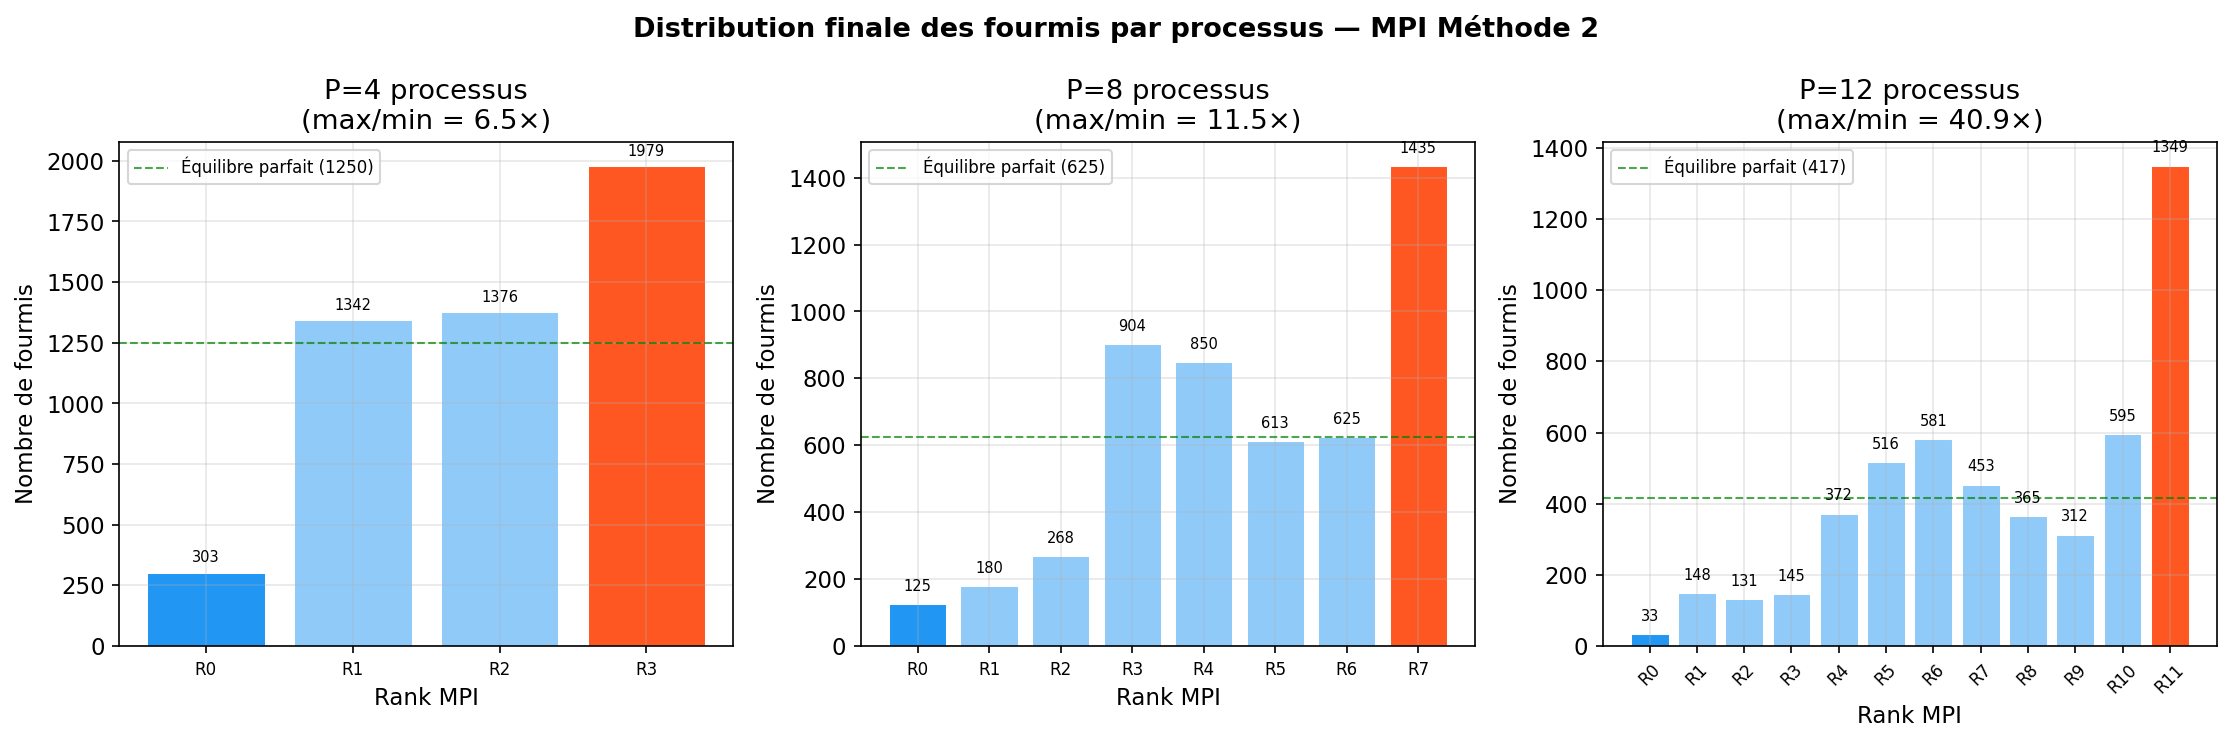
\includegraphics[width=0.78\textwidth]{mpi2_ant_distribution.png}
    \caption{Distribution des fourmis par processus}
    \label{fig:mpi2_ants}
\end{figure}

\subsection{Comparaison méthode 1 vs méthode 2}

\begin{table}[H]
\centering
\begin{tabular}{rrrrr}
\toprule
$\boldsymbol{P}$ & \textbf{M1 (ms)} & \textbf{M2 (ms)} & \textbf{Gain M2/M1} & \textbf{Réduction comm.} \\
\midrule
1  & 10423.50  & 8881.40  & $1.17\times$ & $\times 382$ \\
2  & 9323.80   & 5721.90  & $1.63\times$ & $\times 1.93$ \\
4  & 11655.30  & 3443.80  & $3.38\times$ & $\times 4.07$ \\
8  & 27887.40  & 3216.50  & $\textbf{8.67}\times$ & $\times 10.09$ \\
12 & 112636.50 & 39814.60 & $2.83\times$ & $\times 4.20$ \\
\bottomrule
\end{tabular}
\caption{Comparaison directe méthode 1 vs méthode 2}
\label{tab:m1_vs_m2}
\end{table}

\begin{figure}[H]
    \centering
    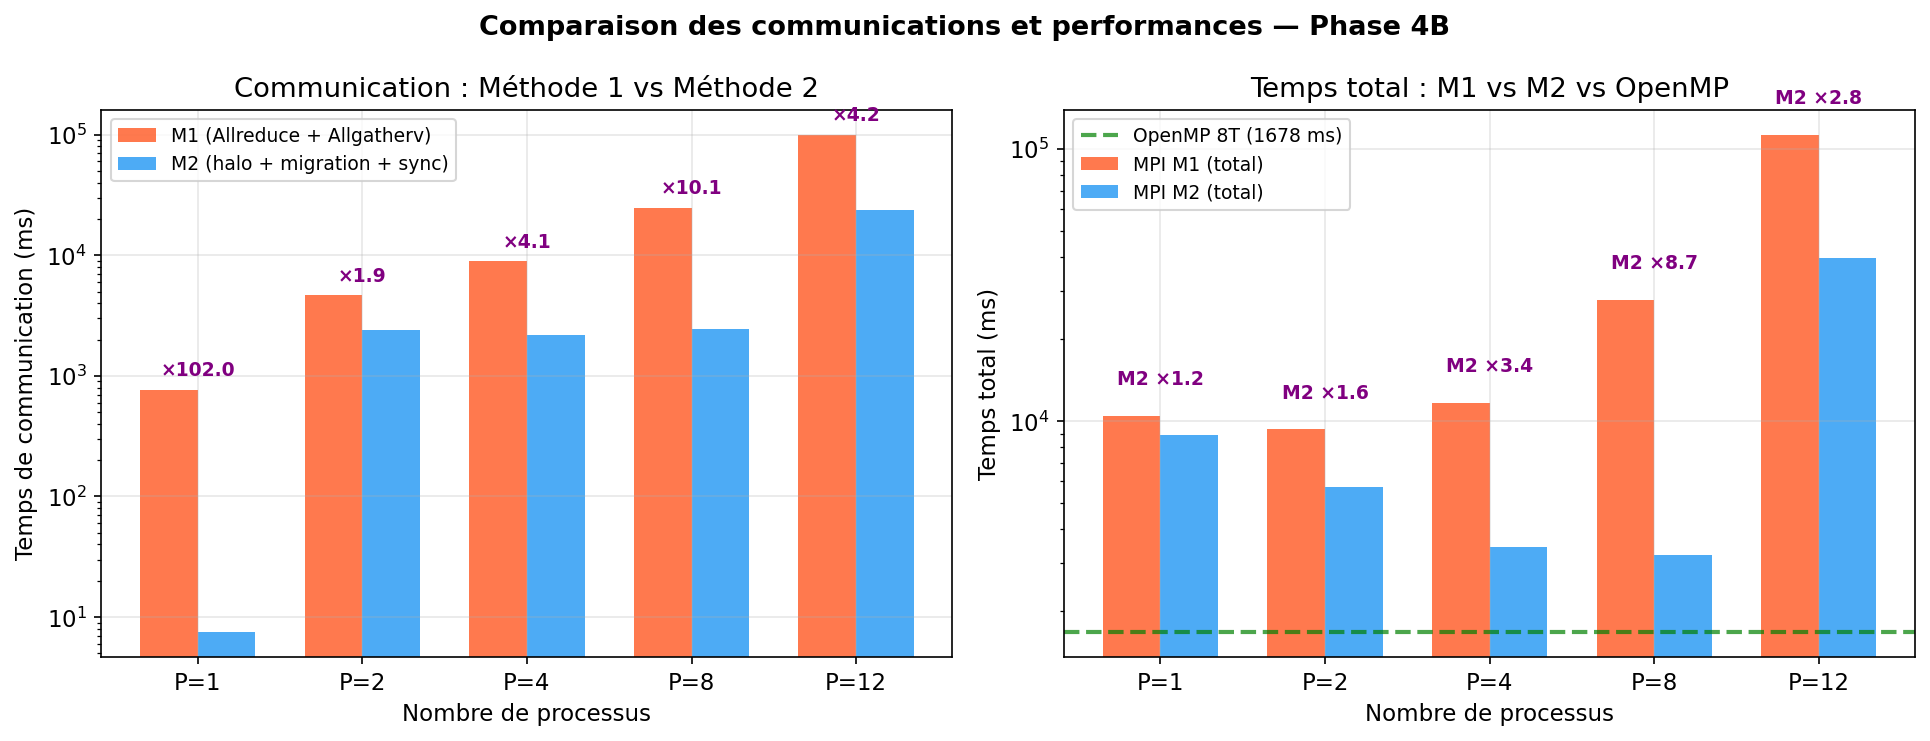
\includegraphics[width=0.78\textwidth]{mpi2_comm_comparison.png}
    \caption{Temps de communication : méthode 1 vs méthode 2}
    \label{fig:mpi2_comm}
\end{figure}

La méthode 2 est systématiquement plus rapide. À $P=8$, elle est $8.67\times$ plus rapide que la méthode 1, grâce à la combinaison de la communication réduite et de l'effet de cache.

\subsection{Convergence algorithmique}

La méthode 2 produit des résultats algorithmiques \textbf{différents} de la version séquentielle pour $P \geq 2$ :

\begin{table}[H]
\centering
\begin{tabular}{lrr}
\toprule
\textbf{Config.} & \textbf{1ère nourriture (iter.)} & \textbf{Nourr. (5000 iter.)} \\
\midrule
Séquentiel / M2 $P=1$ & 2942 & 2440 \\
M2 $P=2$  & 2944 & 2092 \\
M2 $P=4$  & 2672 & 3609 \\
M2 $P=8$  & 2583 & 3445 \\
M2 $P=12$ & 2553 & 3670 \\
\bottomrule
\end{tabular}
\caption{Convergence algorithmique --- MPI méthode 2}
\label{tab:convergence}
\end{table}

Pour $P=1$, M2 reproduit exactement les résultats séquentiels (validation de la correctitude). Pour $P \geq 4$, la première nourriture arrive plus tôt (2672 vs 2942) : le partitionnement de la carte modifie la diffusion des phéromones et crée des raccourcis locaux. Ces différences sont attendues : la méthode 2 est une approximation distribuée de l'algorithme séquentiel.

\subsection{Mode hybride MPI M2 + OpenMP}

\begin{table}[H]
\centering
\begin{tabular}{rrrrrr}
\toprule
$\boldsymbol{P}$ & $\boldsymbol{T}$ & \textbf{Cœurs} & \textbf{Total (ms)} & $\boldsymbol{S_\text{seq}}$ & \textbf{Nourr.} \\
\midrule
1 & 8  & 8  & 8874.60  & $1.03\times$ & 2440 \\
2 & 4  & 8  & 5553.60  & $1.64\times$ & 2092 \\
4 & 2  & 8  & 3316.90  & $2.75\times$ & 3609 \\
3 & 4  & 12 & 4153.00  & $2.19\times$ & 2136 \\
4 & 3  & 12 & 3317.10  & $2.75\times$ & 3609 \\
\textbf{6} & \textbf{2} & \textbf{12} & \textbf{2779.40} & $\textbf{3.28}\times$ & 2103 \\
\bottomrule
\end{tabular}
\caption{Mode hybride MPI M2 + OpenMP ($S_\text{seq} = 9107.10 / T_\text{hybrid}$)}
\label{tab:hybrid}
\end{table}

L'ajout de threads OpenMP intra-processus apporte un gain limité. Pour $P=4$, passer de $T=1$ à $T=2$ ne réduit le temps que de 3.70\%, car le goulot est la synchronisation inter-processus ($\sim$62\% du temps), pas le calcul local. La meilleure configuration hybride est $P=6, T=2$ (2779.40 ms, $3.28\times$), qui bénéficie de bandes étroites (86 lignes, bonne localité cache) et d'une légère accélération OpenMP.


\newpage

% ============================================================
\section{Synthèse et comparaison globale}

\subsection{Classement des 4 approches}

\begin{table}[H]
\centering
\begin{tabular}{clrrrr}
\toprule
\textbf{Rang} & \textbf{Approche} & \textbf{Config.} & \textbf{Temps (ms)} & $\boldsymbol{S}$ \textbf{vs séq.} & \textbf{Cœurs} \\
\midrule
\textbf{1} & \textbf{OpenMP}     & 8 threads   & \textbf{1678.20}  & $\textbf{5.43}\times$ & 8  \\
2 & MPI M2 hybride  & P=6, T=2    & 2779.40  & $3.28\times$ & 12 \\
3 & MPI M2 pur      & P=8         & 3216.50  & $2.83\times$ & 8  \\
4 & OpenMP           & 4 threads   & 2508.00  & $3.63\times$ & 4  \\
5 & MPI M2 hybride  & P=4, T=2    & 3316.90  & $2.75\times$ & 8  \\
6 & MPI M1           & P=2         & 9323.80  & $0.98\times$ & 2  \\
7 & MPI M1           & P=12        & 112636.50 & $0.08\times$ & 12 \\
\bottomrule
\end{tabular}
\caption{Classement des approches (référence séquentielle SoA = 9107.10 ms)}
\label{tab:ranking}
\end{table}

\begin{figure}[H]
    \centering
    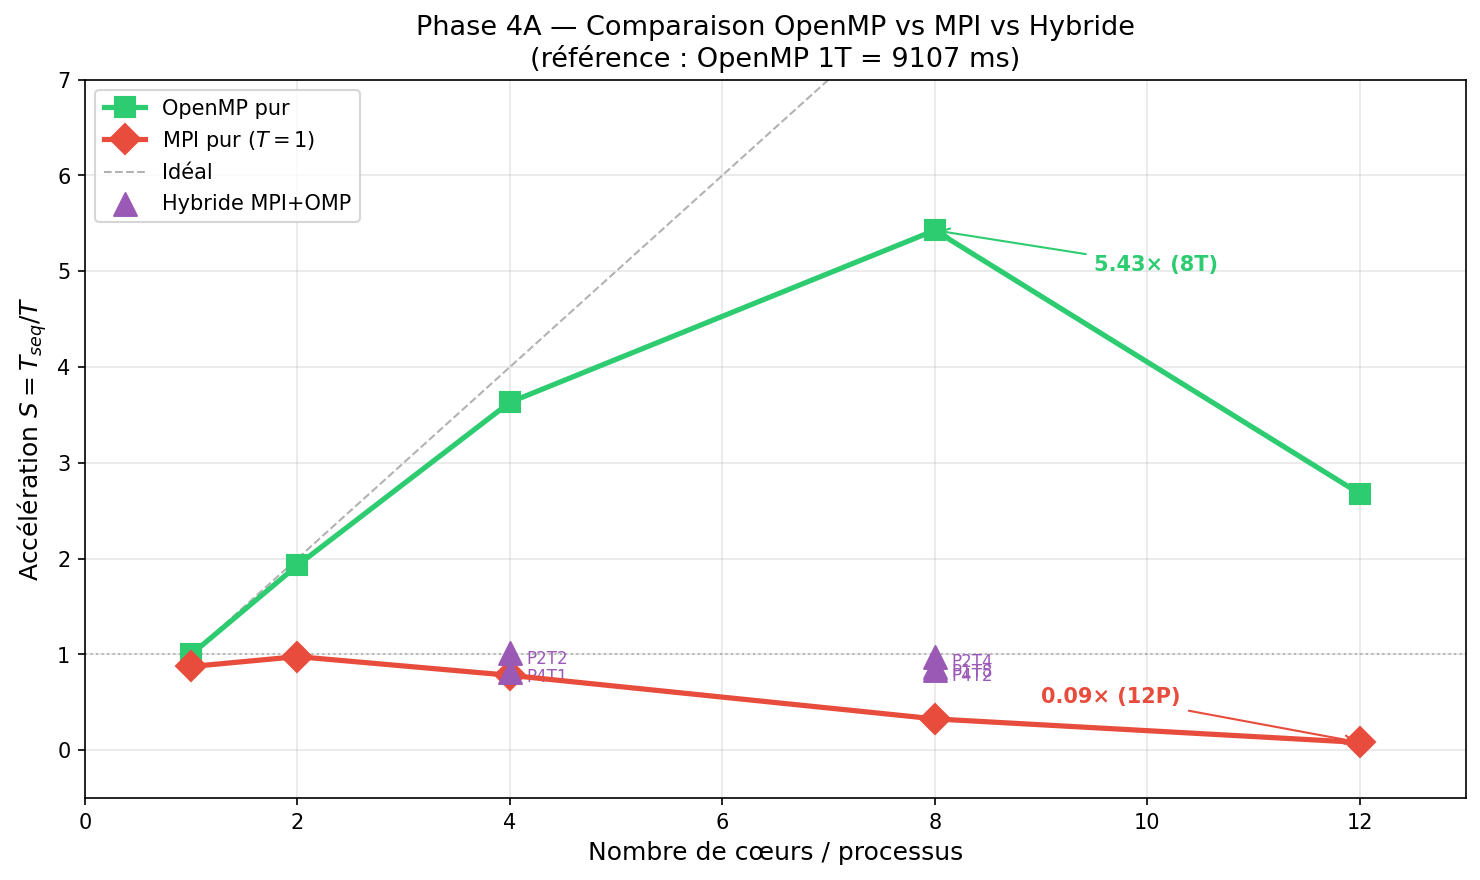
\includegraphics[width=0.78\textwidth]{mpi_vs_omp.png}
    \caption{Comparaison des accélérations : OpenMP vs MPI M1 vs MPI M2 hybride}
    \label{fig:global_comparison}
\end{figure}

\subsection{Analyse comparative}

\begin{table}[H]
\centering
\begin{tabular}{lccc}
\toprule
& \textbf{OpenMP} & \textbf{MPI M1} & \textbf{MPI M2} \\
\midrule
Communication/iter       & 0                  & $\sim$8.50 Mo    & $\sim$50 Ko \\
Équilibre de charge      & Dynamique (bon)    & Statique (bon)   & Statique (mauvais) \\
Effet de cache           & Aucun (4.20 Mo)    & Aucun (4.20 Mo)  & Fort (0.55 Mo à $P=8$) \\
Facteur limitant         & Bande passante mém.& Volume comm.     & Déséquilibre charge \\
Extensibilité multi-nœud & Non                & Oui              & Oui \\
Meilleure accél.         & $5.43\times$ (8T)  & $1.12\times$ (2P)& $3.28\times$ (6P$\times$2T) \\
\bottomrule
\end{tabular}
\caption{Synthèse qualitative des trois approches}
\label{tab:synthesis}
\end{table}

\textbf{Pourquoi OpenMP reste supérieur sur un nœud :} aucune communication, aucune sérialisation de données, pas de migration de fourmis, ordonnancement dynamique avec équilibre de charge automatique. Le seul inconvénient est l'impossibilité de dépasser une machine physique.

\textbf{Pourquoi M2 bat M1 :} la réduction de communication ($\times 170$) et l'effet de cache (carte locale dans L2) compensent largement le déséquilibre de charge. La méthode 2 est la seule approche MPI viable pour cette application.

\textbf{Le compromis fondamental :} la méthode 2 gagne sur le volume de communication mais perd sur l'équilibre de charge. La méthode 1 a un équilibre parfait mais un volume de communication prohibitif. Ni l'une ni l'autre ne bat OpenMP sur un seul nœud, mais seul MPI peut s'étendre sur un cluster multi-nœuds. Pour une telle application distribuée à plus grande échelle, la méthode 2 avec rééquilibrage dynamique des fourmis serait la voie à suivre.

\newpage
% ============================================================
\section*{Conclusion}
\addcontentsline{toc}{section}{Conclusion}

Ce projet a permis d'explorer quatre niveaux d'optimisation d'un simulateur ACO :

\begin{enumerate}[nosep]
    \item \textbf{Vectorisation (SoA)} : gain négligeable (+0.71\%), car le goulot est l'accès aléatoire aux phéromones, pas la disposition des fourmis.
    \item \textbf{OpenMP} : accélération de $5.43\times$ avec 8 threads, limitée par la bande passante mémoire. Régression à 12 threads due à la saturation du bus mémoire lors de l'évaporation.
    \item \textbf{MPI méthode 1} : échec complet (accélération maximale $1.12\times$), dominé par 8.50 Mo/itération de communication collective.
    \item \textbf{MPI méthode 2} : amélioration considérable ($3.28\times$ en hybride), grâce à la communication réduite ($\sim$50 Ko/itération) et à l'effet de cache super-linéaire. Limitée par le déséquilibre de charge (ratio $40.88 \times$ à $P=12$).
\end{enumerate}

Le résultat principal est que, sur un seul nœud, la parallélisation en \textbf{mémoire partagée} (OpenMP) surpasse systématiquement la parallélisation \textbf{distribuée} (MPI), car l'overhead de communication et de synchronisation domine dès que le ratio calcul/communication est défavorable. La méthode 2 démontre néanmoins l'intérêt du partitionnement de données pour les applications à empreinte mémoire importante : l'effet de cache (accélération super-linéaire des fourmis, $22.51\times$ à $P=8$) constitue un avantage structurel qui pourrait être décisif sur un cluster multi-nœuds avec des grilles de plus grande taille.

% ============================================================
\newpage
\appendix
\section{Guide de reproduction des expériences}

\subsection{Prérequis}

Les expériences ont été réalisées sur une VM OrbStack Ubuntu 22.04 (aarch64, 12 cœurs ARM). Les dépendances nécessaires sont :

\begin{lstlisting}[language=bash, caption={Installation des dépendances}]
sudo apt update
sudo apt install -y build-essential g++ libsdl2-dev \
    openmpi-bin libopenmpi-dev
\end{lstlisting}

Vérifier les versions :
\begin{itemize}[nosep]
    \item \texttt{g++ --version} $\rightarrow$ GCC 11.4.0 ou supérieur
    \item \texttt{mpic++ --version} $\rightarrow$ OpenMPI wrapping GCC
    \item \texttt{sdl2-config --version} $\rightarrow$ SDL2 2.0.x
\end{itemize}

\subsection{Compilation}

Le fichier \texttt{Make\_linux.inc} contient la configuration du compilateur :
\begin{lstlisting}[language=bash, caption={Compilation de toutes les cibles}]
cd projet/src
make clean && make all
\end{lstlisting}

Ceci génère les exécutables suivants :
\begin{itemize}[nosep]
    \item \texttt{ant\_simu.exe} --- version séquentielle originale (AoS)
    \item \texttt{ant\_simu\_soa.exe} --- version SoA
    \item \texttt{ant\_simu\_omp.exe} --- version OpenMP (SoA)
    \item \texttt{ant\_simu\_mpi.exe} --- MPI méthode 1
    \item \texttt{ant\_simu\_mpi2.exe} --- MPI méthode 2 (partitionnement)
\end{itemize}

\subsection{Exécution des expériences}

\subsubsection{Baseline et SoA}

\begin{lstlisting}[language=bash, caption={Mesure de la baseline et SoA}]
# Baseline (3 runs)
for i in 1 2 3; do
    ./ant_simu.exe --headless -n 5000
done 2>&1 | tee ../results/baseline_3runs.txt

# SoA (3 runs)
for i in 1 2 3; do
    ./ant_simu_soa.exe --headless -n 5000
done 2>&1 | tee ../results/soa_3runs.txt
\end{lstlisting}

\subsubsection{OpenMP}

\begin{lstlisting}[language=bash, caption={Passage à l'échelle OpenMP}]
for T in 1 2 4 8 12; do
    for i in 1 2 3; do
        ./ant_simu_omp.exe --headless -n 5000 -t $T
    done
done 2>&1 | tee ../results/omp_scaling.txt
\end{lstlisting}

\subsubsection{MPI méthode 1}

\begin{lstlisting}[language=bash, caption={Passage à l'échelle MPI méthode 1}]
for P in 1 2 4 8 12; do
    for i in 1 2 3; do
        mpirun -np $P --oversubscribe \
            ./ant_simu_mpi.exe --headless -n 5000 -t 1
    done
done 2>&1 | tee ../results/mpi_scaling.txt
\end{lstlisting}

\subsubsection{MPI méthode 2}

\begin{lstlisting}[language=bash, caption={Passage à l'échelle MPI méthode 2}]
# MPI M2 pur
for P in 1 2 4 8 12; do
    for i in 1 2 3; do
        mpirun -np $P --oversubscribe \
            ./ant_simu_mpi2.exe --headless -n 5000 -t 1
    done
done 2>&1 | tee ../results/mpi2_scaling.txt

# MPI M2 hybride
for P in 1 2 3 4 6; do
    for T in 2 4; do
        for i in 1 2 3; do
            mpirun -np $P --oversubscribe \
                ./ant_simu_mpi2.exe --headless -n 5000 -t $T
        done
    done
done 2>&1 | tee ../results/mpi2_omp_hybrid.txt
\end{lstlisting}

\subsection{Génération des graphiques}

Trois scripts Python (nécessitant \texttt{matplotlib} et \texttt{numpy}) sont fournis dans \texttt{results/} :

\begin{lstlisting}[language=bash, caption={Génération des figures}]
cd projet/results
python3 plot_omp_scaling.py     # -> omp_*.png
python3 plot_mpi_scaling.py     # -> mpi_*.png
python3 plot_mpi2_results.py    # -> mpi2_*.png
\end{lstlisting}

\subsection{Liste des fichiers nécessaires}

Pour la reproductibilité complète, les fichiers suivants doivent être inclus :

\begin{table}[H]
\centering
\begin{tabular}{lll}
\toprule
\textbf{Catégorie} & \textbf{Fichier} & \textbf{Rôle} \\
\midrule
\multirow{5}{*}{Sources C++}
    & \texttt{src/ant\_simu.cpp}      & Baseline séquentielle \\
    & \texttt{src/ant\_simu\_soa.cpp}  & Version SoA \\
    & \texttt{src/ant\_simu\_omp.cpp}  & Version OpenMP \\
    & \texttt{src/ant\_simu\_mpi.cpp}  & MPI méthode 1 \\
    & \texttt{src/ant\_simu\_mpi2.cpp} & MPI méthode 2 \\
\midrule
\multirow{10}{*}{Headers}
    & \texttt{src/ant.hpp}             & Classe ant (AoS) \\
    & \texttt{src/ant.cpp}             & Implémentation ant \\
    & \texttt{src/ant\_soa.hpp}        & Structure SoA \\
    & \texttt{src/ant\_soa\_omp.hpp}   & SoA + OpenMP \\
    & \texttt{src/pheronome.hpp}       & Carte de phéromones \\
    & \texttt{src/fractal\_land.hpp/cpp} & Terrain fractal \\
    & \texttt{src/renderer.hpp/cpp}    & Rendu SDL2 \\
    & \texttt{src/window.hpp/cpp}      & Fenêtre SDL2 \\
    & \texttt{src/basic\_types.hpp}    & Types de base \\
    & \texttt{src/rand\_generator.hpp} & Générateur aléatoire \\
\midrule
\multirow{2}{*}{Build}
    & \texttt{src/Makefile}            & Fichier de compilation \\
    & \texttt{src/Make\_linux.inc}     & Config. Linux \\
\midrule
\multirow{3}{*}{Scripts}
    & \texttt{results/plot\_omp\_scaling.py}  & Graphiques OpenMP \\
    & \texttt{results/plot\_mpi\_scaling.py}  & Graphiques MPI M1 \\
    & \texttt{results/plot\_mpi2\_results.py} & Graphiques MPI M2 \\
\midrule
\multirow{2}{*}{Données}
    & \texttt{results/*.txt}           & Données brutes \\
    & \texttt{results/*.png}           & Figures générées \\
\midrule
Rapport
    & \texttt{rapport.pdf}            & Rapport \\
\bottomrule
\end{tabular}
\caption{Fichiers nécessaires à la soumission}
\label{tab:files}
\end{table}

\begin{thebibliography}{9}
\bibitem{cours}
Supports de cours OS02, ENSTA Paris, 2026.

\bibitem{aco}
M.~Dorigo et T.~St\"utzle, \emph{Ant Colony Optimization}, MIT Press, 2004.

\bibitem{amdahl}
G.~M.~Amdahl, ``Validity of the single processor approach to achieving large scale computing capabilities'', \emph{AFIPS Conference Proceedings}, vol.~30, pp.~483--485, 1967.
\end{thebibliography}

\end{document}
